\iffalse \bibliography{MGymrekRefs.bib} \fi

\chapter{Worldwide variation in human short tandem repeats}

\label{chap:sgdp}

\hzline

Parts of this chapter have been submitted to \emph{Nature} for publication:
\begin{itemize}
\item[] Mallick S, Li H, Lipson M, Mathieson I, \textbf{Gymrek M}, \emph{et al.}. The landscape of human diveristy. Under revision.
\end{itemize}
The STR work is mostly described in a supplemental chapter to this work:
\begin{itemize}
\item[] \textbf{Gymrek M}, Willems TF, Reich D, Erlich Y. Worldwide variation in human short tandem repeats. 
\end{itemize}
\hzline

\textbf{Summary:} We generated the most comprehensive catalog of short tandem repeat (STR) genotypes to date, based on 301 deeply sequenced human genomes. Genotypes show strong concordance with capillary electrophoresis and accurately recover population structure. We used this call set to characterize allele frequency spectra, analyze sequence determinants of STR variation, and to identify common loss of function alleles. STR genotypes are available in raw and interactive format at \url{strcat.teamerlich.org}.

\begin{figure}[h!]
\centering
\label{fig:sgdped}
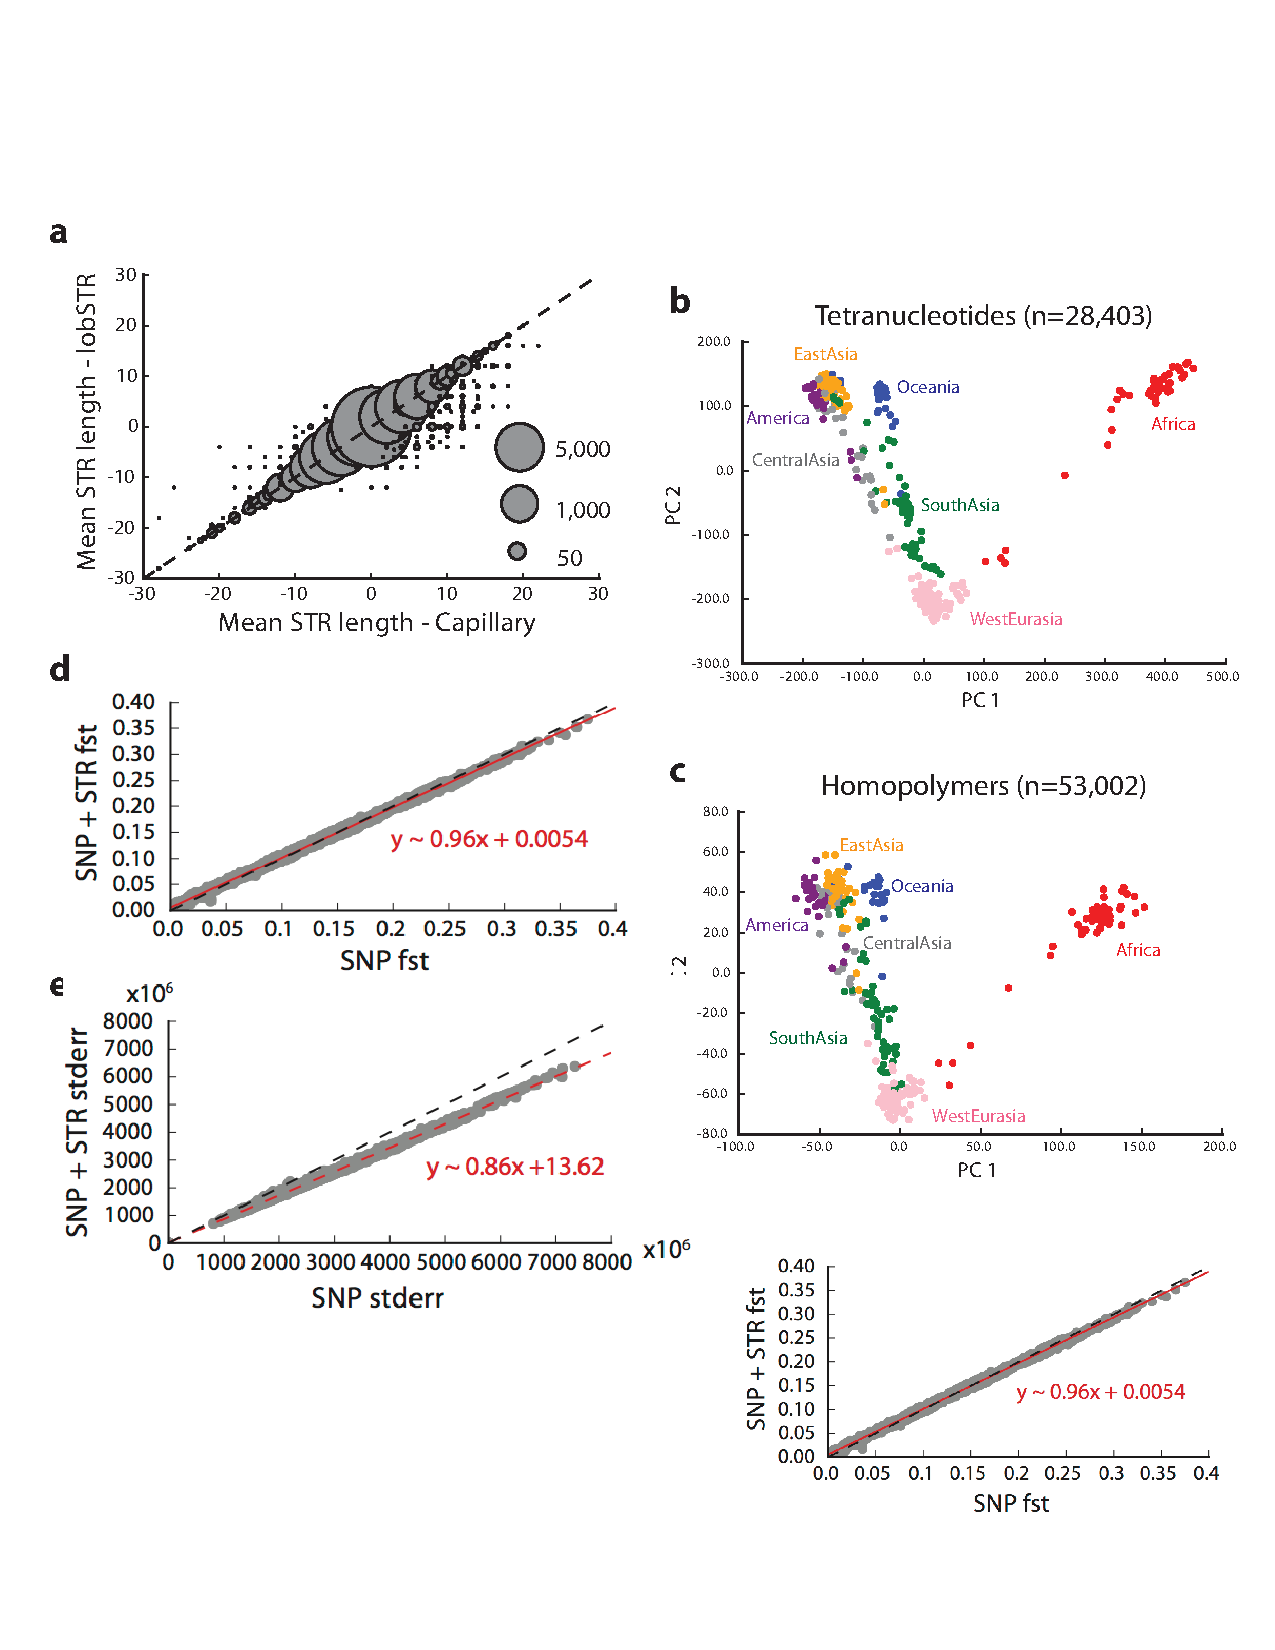
\includegraphics[width=0.8\textwidth]{Figures/App3/FigED.pdf}
\caption{\textbf{Worldwide variation in human short tandem repeats.} \textbf{a.} Mean STR length is reported as the average of the length difference (in bp) from the GRCh37 reference for each genotype. Bubble area scales with the number of calls compared at each point. \textbf{b.} and \textbf{c.} show the first two principal components after performing principal component analysis on tetranucleotide and homopolymer genotypes, respectively. Colors represent the region of origin of each sample. \textbf{d.} Pairwise Fst values between populations computed using only SNPs vs. using combined SNP+STR loci. \textbf{e.} Block jackknife standard errors for the SNP vs. SNP+STR $F_{ST}$ analysis. The red dashed lines give the best-fit line, described by the formula in red. The black dashed line denotes the diagonal.}
\end{figure}

\section{Genotyping STRs}
We analyzed STRs using lobSTR \cite{GymrekGolanRossetEtAl2012}, a custom algorithm for genotyping short tandem repeats. We modified lobSTR's allelotyping tool to be able to call STRs directly from alignments generated by tools besides the lobSTR aligner. This greatly reduces the run time and allows rapid STR genotyping from large sequencing panels that have already been aligned using alternative indel-sensitive methods. We used raw reads aligned to GRCh37 using BWA-MEM (\url{http://bio-bwa.sourceforge.net/}) (version 0.7.10) with default parameters. These alignments were used as input to lobSTR's allelotyper (Github revision 3.0.3.24-892e). We used optional parameters ``-{}-filter-mapq0 -{}-filter-clipped -{}-max-repeats-in-ends 3 -{}-min-read-end-match 10'' and a noise model trained on PCR-free sequencing data. We jointly genotyped samples at sites in lobSTR's reference panel: 1.6 million loci with motif lengths ranging from 1-6bp. The reference is part of the GRCh37 lobSTR resource bundle available at \url{http://lobstr.teamerlich.org/download.html}. \textbf{Table \ref{tab:sgdptab1}} provides a summary of the reference panel.

\section{Quality controls}
lobSTR generated genotypes for an average of 1.5 million loci per sample (\textbf{Figure \ref{fig:sgdpfig1}a}) with an average of 15.3 informative reads (reads that completely span the repeat region) for each autosomal call. We removed sample S\_Daur-1 from analysis because it had 6.5 standard deviations fewer calls than the mean (1.4 million calls). All other samples were within 3 standard deviations of the mean. For downstream population genetic analysis, we also removed individuals from the Bergamo and Hazara populations, as some of these individuals were outliers. Each locus had genotype calls for an average of 280 samples (95\%) (\textbf{Figure \ref{fig:sgdpfig1}b}). We were not able to genotype 2\% of loci in our reference. Most of these loci have allele lengths greater than 100bp that could not be spanned by Illumina reads. Genotype quality scores, which report the likelihood of the genotype call divided by the sum of likelihoods of all considered genotypes, tended to decrease for longer STRs and increase with motif length, with homopolymers showing significantly lower quality scores than other classes (\textbf{Figure \ref{fig:sgdpfig1}c}). For the majority of loci, we found no directional bias in allele length compared to the reference allele. However, as the reference track increases, calls become biased toward shorter alleles, again reflecting the limitation of calling STR genotypes using 100bp reads ((\textbf{Figure \ref{fig:sgdpfig1}d})).

\begin{figure}[h!]
\centering
\label{fig:sgdpfig1}
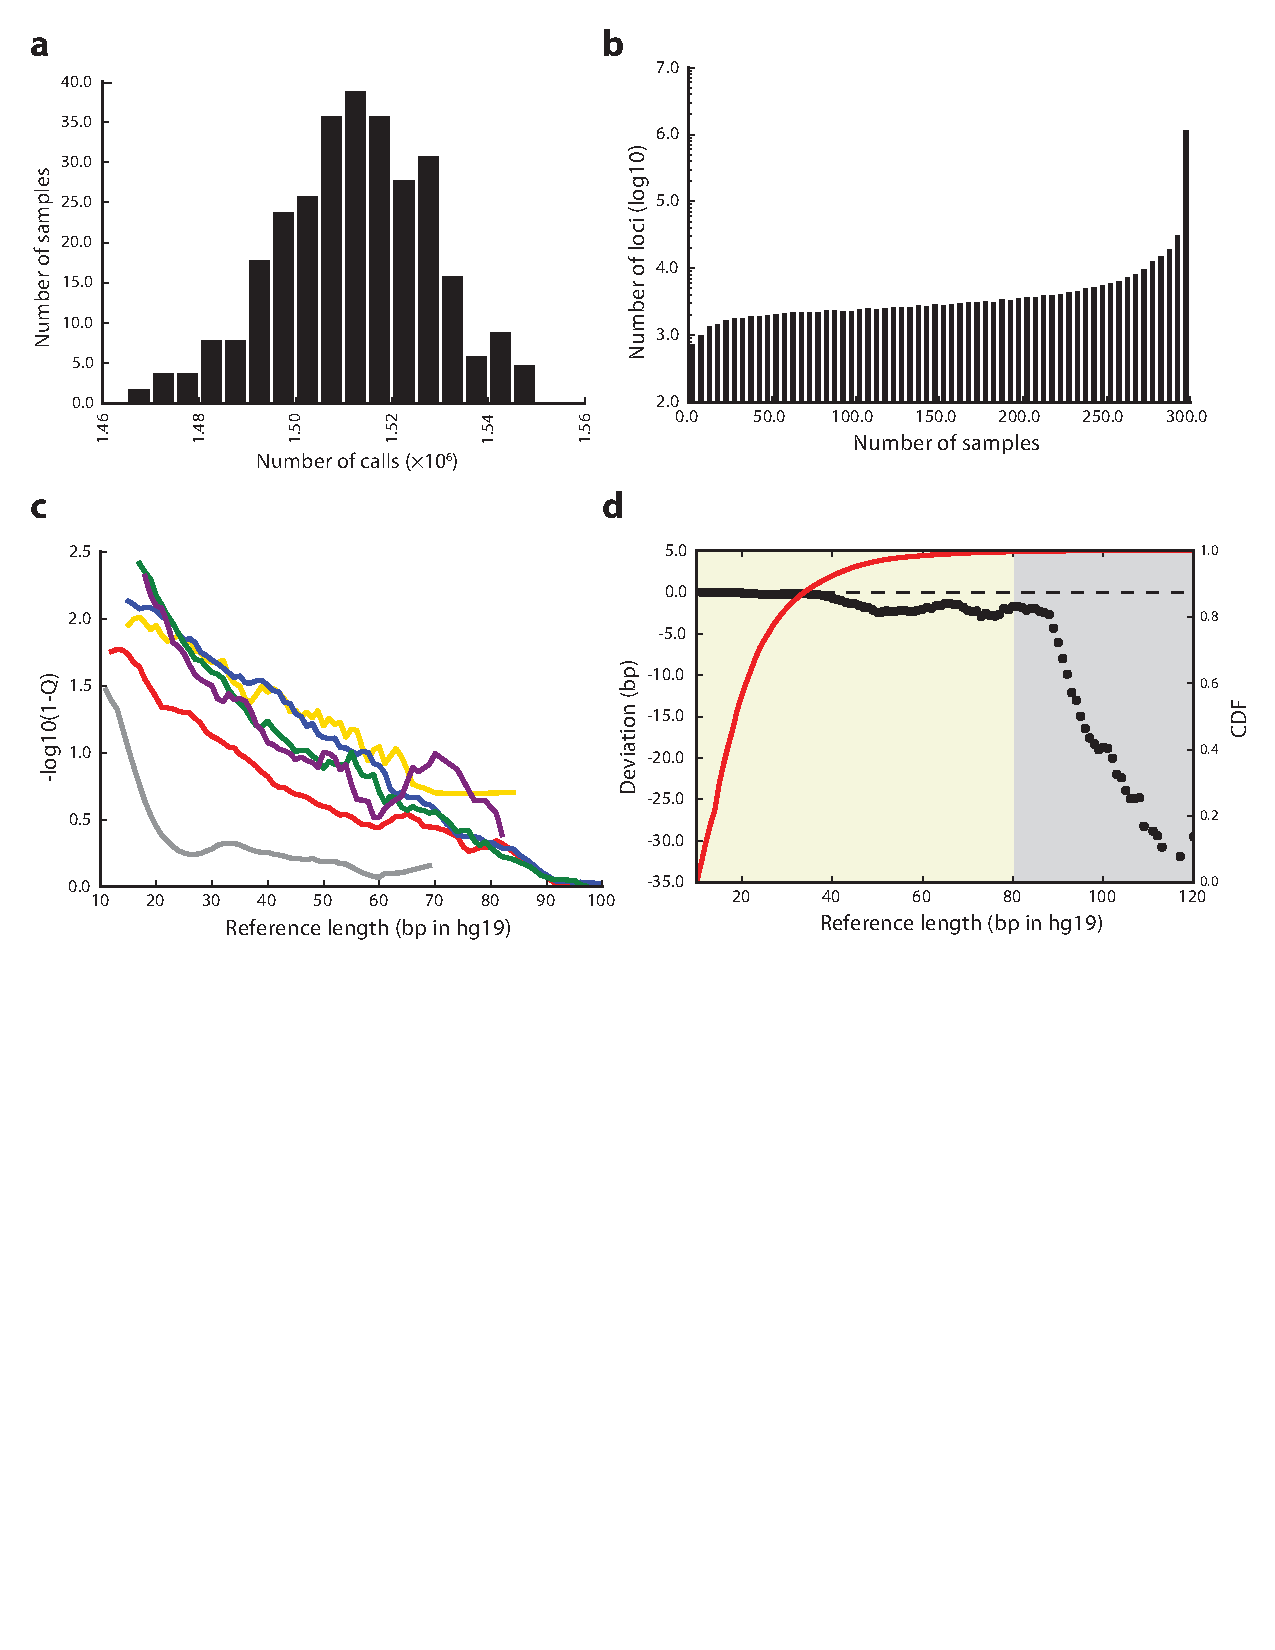
\includegraphics[width=0.8\textwidth]{Figures/App3/Fig1.pdf}
\caption{\textbf{STR call set quality metrics.} \textbf{a}. Distribution of the number of STR calls per sample. \textbf{b}. Distribution of the number of samples with calls for each STR. \textbf{c}. Mean genotype quality score decreases with the length of the STR. Each line represents a different repeat motif length (gray = homopolymers, red = dinucleotides, yellow = trinucleotides, blue = tetranucleotides, green = pentanucleotides, purple = hexanucleotides). \textbf{d}. Mean length deviation from the reference allele as a function of reference length (black). As the reference track increases in length, calls tend to be biased toward alleles shorter than the reference allele (black). The red line gives the Cumulative Distribution Function (CDF) of calls vs. reference length. Gray shading: loci that were filtered from analysis. Beige: loci retained for downstream analysis.}
\end{figure}

We subjected the resulting genotypes to stringent filtering to ensure high quality calls. We based our filters on coverage, call rate (percent of samples with a genotype call for a given locus), and the metrics Q and DISTENDS reported in the VCF file generated by lobSTR. Q reports the genotype quality score as described above. DISTENDS reports the mean distance between the STR boundary and the end of the read. Specifically, we calculate the difference in distance between the STR and the left and right read ends, and take the average difference across all reads for a given call. We find that high quality calls tend to have DISTENDS close to 0, meaning there is no bias towards a specific end of the read on which the STR occurs. On the other hand large positive or negative DISTENDS scores often indicate that a locus has problematic alignments.

\begin{table}[h!]
\centering
\label{tab:sgdptab1}
\begin{adjustbox}{width=1\textwidth}
\begin{tabular}{l l l l l}
\hline
Motif length & No. of loci & \% in reference & Common motifs & \% genotyped (post-filtering) \\
\hline
1	& 795,043	& 48.5	& A, C	& 99.9 (70.3) \\
2	& 310,761	& 19.0	& AC, AT, AG& 	96.2 (88.5) \\
3	& 84,869	& 5.2	& AAT, AAC, AGG, AAG, ATC &	97.6 (95.6) \\
4	& 262,179	& 16.0	& AAAT, AAAC, AAAG, AAGG, AATG, AGAT, AGGG, ATCC, ACAT	& 94.3 (91.8) \\
5	& 106,481	& 6.5	& AAAAC, AAAAT, AAAAG	& 97.4 (93.1)\\
6	& 79,246	& 4.8	& AAAAAC, AAAAAT, AAAAAG	& 97.4 (93.3) \\
All &	1,638,516	& 100.0	&	& 97.9 (81.1) \\
\hline
\end{tabular}
\end{adjustbox}
\caption{\textbf{Composition of GRCh37 lobSTR reference panel.} We list motifs that occur $>$5,000 times in the reference, in order from most to least common.}
\end{table}

The specific filters listed below are described in the ``Best practices for using BWA-MEM alignments with lobSTR'' section of the lobSTR website. We filtered loci with the following properties:

\begin{itemize}
\item Average coverage $5 \times$
\item Average $-\log_{10}(1-Q)<0.8$
\item Call rate $<0.8$
\item Reference allele length $>$80bp
\end{itemize}

After filtering loci we additionally filtered individual calls with:

\begin{itemize}
\item Coverage $<5 \times$
\item $-\log_{10}(1-Q)<0.8$
\item Absolute value of DISTENDS score $>$20
\end{itemize}
After filtering, 1.3 million loci remained for analysis.

\section{Validation}
We compared lobSTR results to genotypes for a subset of samples generated using capillary electrophoresis, the gold standard for STR genotyping. We evaluated concordance with two panels: Y chromosome STRs (mostly tetranucleotide loci), and the Marshfield set of mostly di- and tetranucleotide autosomal loci.

We obtained Y-STR genotypes for 74 samples at 39 loci that overlapped with our data from the CEPH website (\url{ftp://ftp.cephb.fr/hgdp_supp9/genotype-supp9.txt}). We calibrated capillary calls to the lobSTR format using the reference alleles annotated in Supplementary Table 5 of Gymrek et al. \cite{GymrekMcGuireGolanEtAl2013}. As reported there, markers DYS481 and DYS594 are off by one unit in the CEPH data, and we corrected the lobSTR calls to reflect this. We discarded marker DYS640 due to ambiguous nomenclature. We found overall concordance of 99\% between the lobSTR and capillary calls. 

\begin{figure}[h!]
\centering
\label{fig:sgdpfig2}
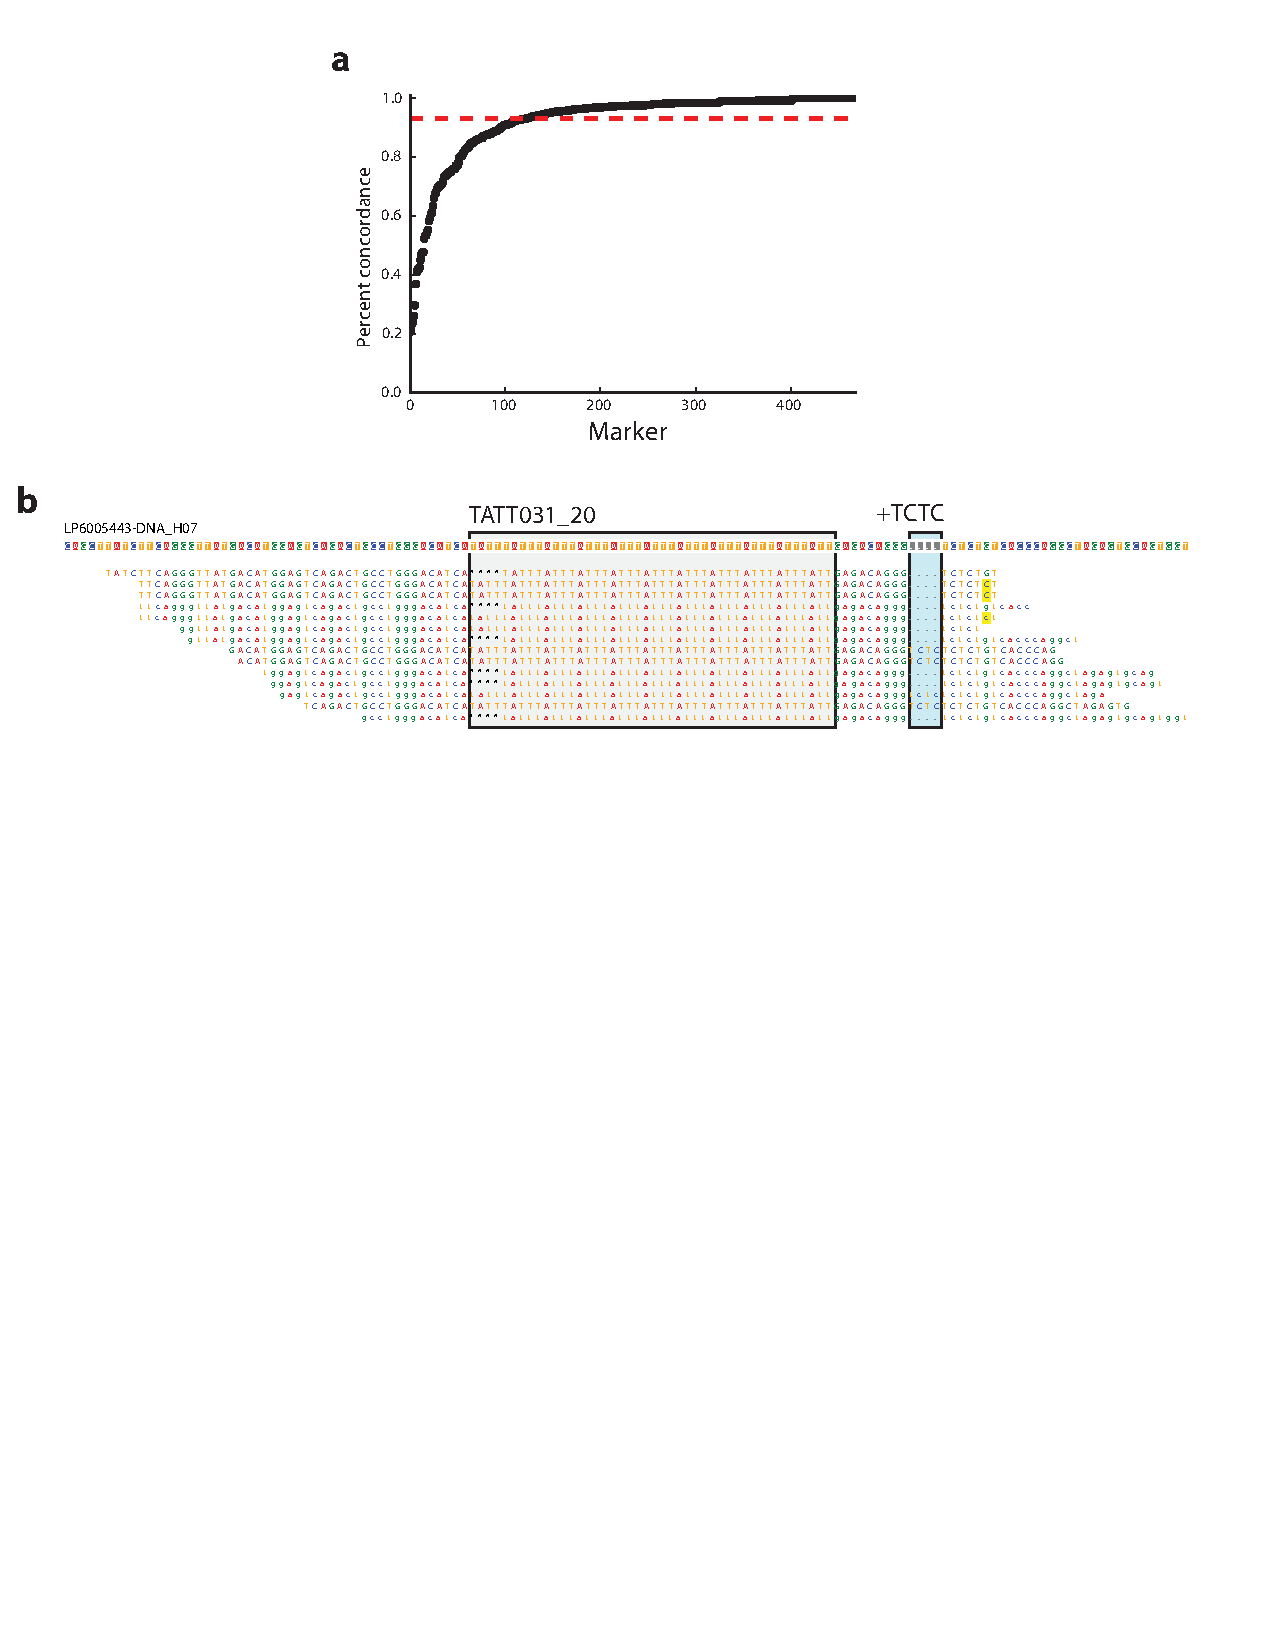
\includegraphics[width=0.8\textwidth]{Figures/App3/Fig2.pdf}
\caption{\textbf{Concordance between lobSTR and capillary genotypes.} \textbf{a}. Concordance by marker, ordered from the marker with lowest to highest concordance. The red dashed line gives the overall concordance. \textbf{b}. Example marker with poor concordance between lobSTR and capillary data due to an annotation error. In this sample, marker TATT031\_20 has a genotype of -4,0 reported by lobSTR. However, the capillary data reports -4,4, due to an extra 4bp TCTC indel (blue box) in the flanking regions that is linked with the STR allele 0. Because this indel is not included in the annotated STR sequence (gray box) lobSTR does not consider it when making a genotype call. We visualized the alignment using PyBamView \cite{Gymrek2014}.}
\end{figure}

We downloaded genotypes and additional metadata for the Marshfield markers for 1,048 samples at 627 loci from the Rosenberg lab website as reported by Pemberton et al. \cite{PembertonSandefurJakobssonEtAl2009}. A total of 127 of these samples overlapped between our sequencing and this capillary dataset, and of these, we were able to convert 468 capillary genotyped loci to loci in the lobSTR GRCh37 reference. Capillary genotypes were reported as the size of the PCR product and we converted these to lobSTR format as described on the lobSTR webpage. We rounded all genotypes to the nearest repeat unit. The overall concordance rate was 93\%. We compared STR dosage, defined as the sum of lengths of the two alleles, across methods and found strong correlation ($r^2=0.92$) between the two datasets (\textbf{Figure \ref{fig:sgdped}a}). In discrepant calls, lobSTR tended to underestimate the true allele length compared to the capillary data, again reflecting a bias toward detecting shorter alleles due to the read length limitation. Notably, the majority of errors originated from a small set of loci (\textbf{Figure \ref{fig:sgdpfig2}a}), with many errors potentially due to discrepancies in STR annotations between the datasets. For instance, marker TATT031\_20 has a 4bp indel nearby the annotated STR sequence that is strongly linked to particular STR alleles. lobSTR only considers variation within the annotated sequence when making calls, whereas the capillary calls consider all length variation contained in the product amplified by PCR during genotyping, resulting in discordant genotypes. Thus, both methods are correct by their own definitions, despite the apparent discrepancy. An example discordant call affected by this issue is shown in \textbf{Figure \ref{fig:sgdpfig2}b}. 

We next sought to assess the accuracy of homopolymers in our data. These markers are not part of the capillary data discussed above and were excluded in previous studies of STR variation \cite{WillemsGymrekHighnamEtAl2014}. To this end, we tested whether the lobSTR calls from these loci could recapitulate known differences between population groups based on principal component analysis (PCA). As a positive control, we first analyzed autosomal tetranucleotides with heterozygosity greater than 10\% that were called in at least 90\% of samples. These loci represent a relatively high quality STR call-set. The 28,403 tetranucleotides passing the above filters were able to accurately recover known population differences in these samples (\textbf{Figure \ref{fig:sgdped}b}), with the first principal component separating non-African from African samples and the second primarily separating European and Asian samples. Remarkably, repeating the same analysis with 53,002 homopolymer loci, we were able to recover the majority of the structure seen by tetranucleotides (\textbf{Figure \ref{fig:sgdped}d}), a testament to the quality of the calls in our catalog for these difficult-to-genotype loci.

\section{STRs improve resolution of population structure inference}
Encouraged by the ability of STR calls to distinguish population structure, we sought to determine whether STRs increase the resolution of population inference beyond that which can be obtained by genome-wide SNPs. We used the smartpca tool from the EIGENSOFT \cite{PricePattersonPlengeEtAl2006} package to compute $F_{ST}$ and block jackknife standard errors between all pairs of populations. We first computed $F_{ST}$ and standard errors using SNPs. Genotypes were pulled down for 1,152,838 autosomal sites from a panel of SNPs known to be informative for population structure, built from a union of panels 1 and 2 of an existing dataset \cite{FuHajdinjakMoldovanEtAl2015}. We then repeated this analysis using a dataset that combined SNP and STR genotype data. To encode STRs in bi-allelic format, we followed the convention suggested by Patterson et al. \cite{PattersonPriceReich2006}, and encoded each STR allele in the frequency range of 5-95\% as a separate bi-allelic marker. This gave 357,863 STR ``markers'' from 160,530 unique STR loci for a total of 1.51 million markers for the combined SNP+STR analysis. Whereas the two datasets gave highly concordant $F_{ST}$ values (slope of best fit line = 0.96, Pearson $r^2=0.999$) (\textbf{Figure \ref{fig:sgdped}d}), the combined dataset has decreased standard errors compared to SNP variation alone (slope = 0.86), documenting the added value provided by STRs for discerning population structure (\textbf{Figure \ref{fig:sgdped}e}).

\section{Patterns of STR variation}
We used our catalog to examine overall trends in polymorphism at STRs. Of the 1.3 million genotyped loci, 32.2\% show more than two common alleles (defined as having an allele frequency $\geq$ 0.01), and some loci have more than 20 common alleles. The remaining loci are either fixed across all individuals (47.6\%) or have only two common alleles (20.5\%). These patterns changed significantly when stratifying by motif length, with longer motif lengths showing less variability. For instance, only 23\% of homopolymers are fixed compared to 70\% of tetranucleotides (\textbf{Figure \ref{fig:sgdpfig3}}). 

\begin{figure}[h!]
\centering
\label{fig:sgdpfig3}
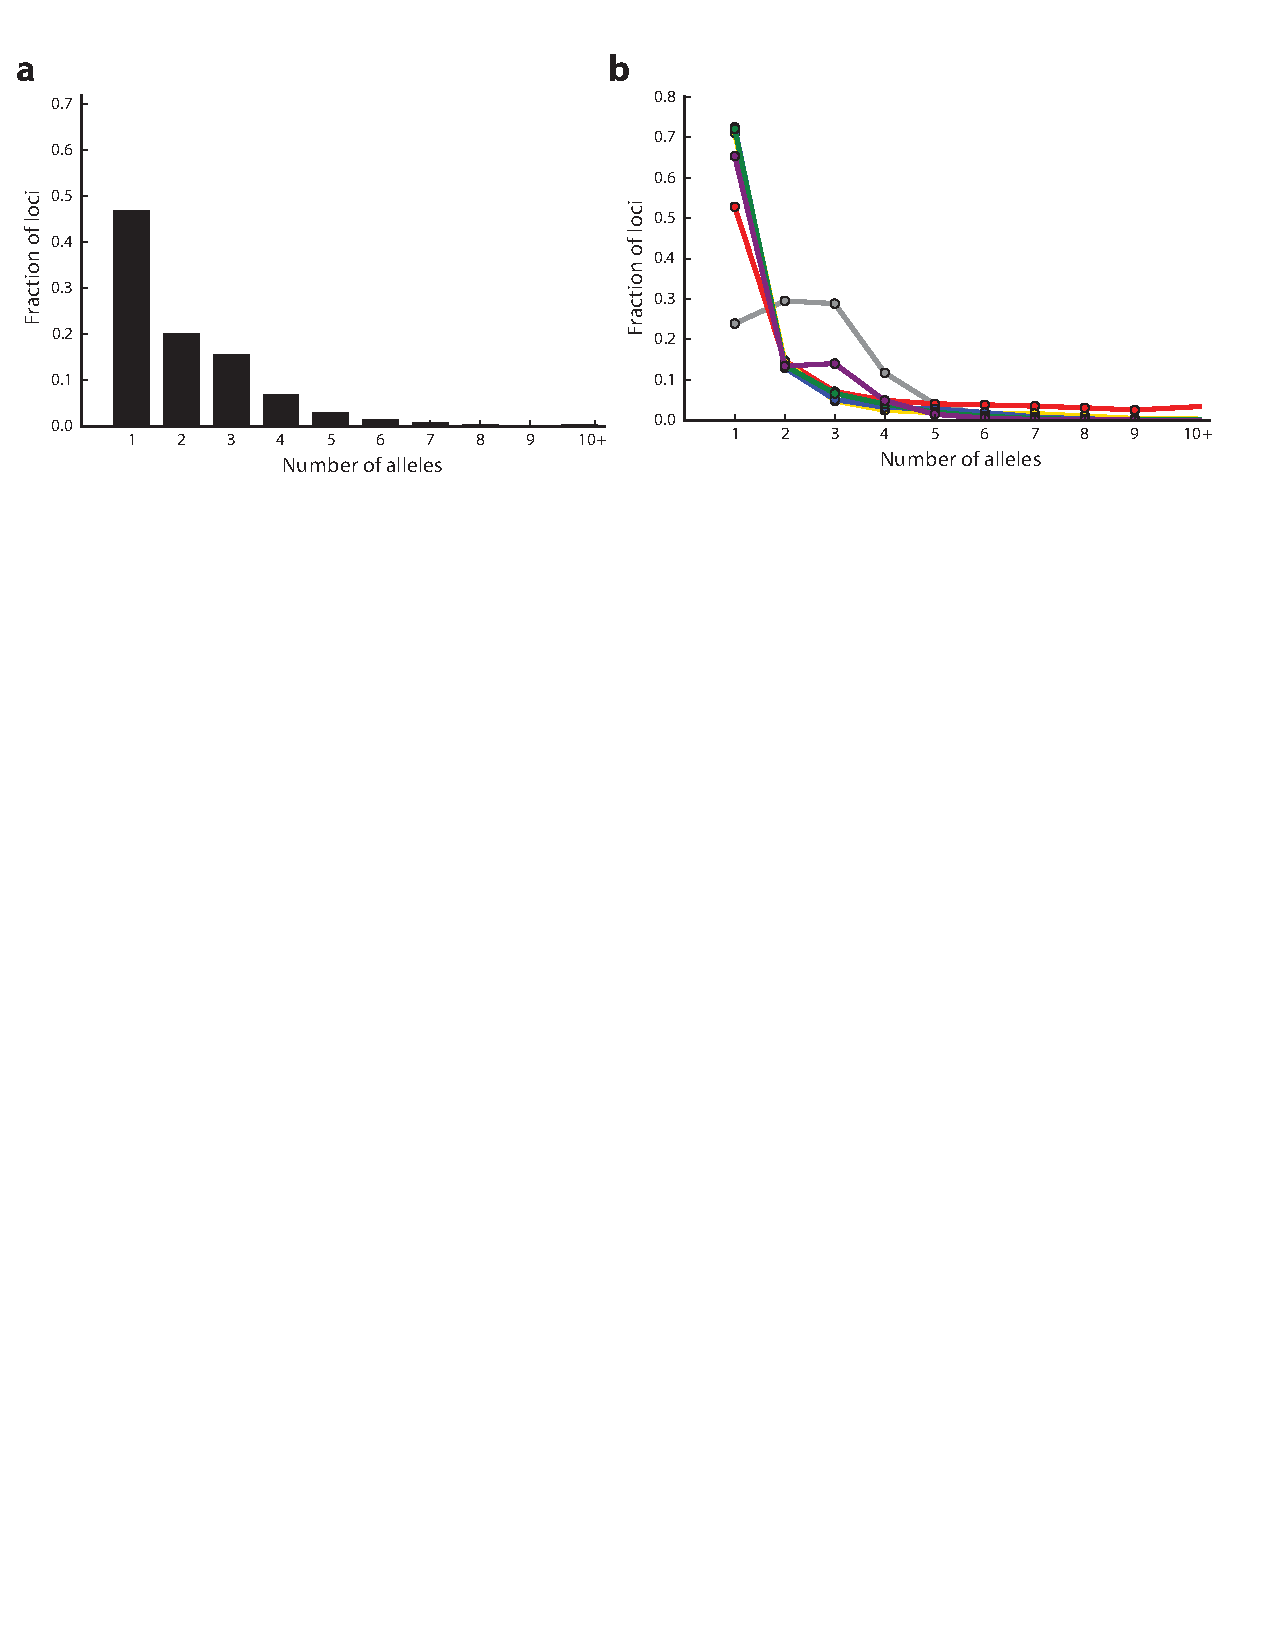
\includegraphics[width=0.8\textwidth]{Figures/App3/Fig3.pdf}
\caption{\textbf{Allele frequency spectra of STRs.} \textbf{a}. Distribution of the number of common alleles per locus. \textbf{b}. Stratification by motif length (gray=homopolymers, red = dinucleotides, yellow = trinucleotides, blue = tetranucleotides, green = pentanucleotides, purple = hexanucleotides).}
\end{figure}

As has been previously shown, we found that STR variability depends strongly on properties of the STR itself and on local sequence features. We examined the ability of these features to explain differences in variability for all STR loci with at least two common alleles. We used heterozygosity as a metric of variation, which is defined as $1-\sum_{i=1}^n p_i^2$ , where $p_i$  is the frequency of allele $i$ and $n$ is the total number of alleles. As mentioned above, heterozygosity tends to decrease with motif length. Additionally, we found that heterozygosity is positively correlated with STR sequence purity ($r = 0.21, p<10^{-200}$) and reference track length ($r = 0.17, p<10^-{200}$) (\textbf{Figure \ref{fig:sgdpfig4}}). Both these observations agree with previously reported results \cite{WillemsGymrekHighnamEtAl2014,ODushlaineShields2008}. We also observed a positive correlation with local recombination rate ($r = 0.028, p=7.4\times 10^{-209}$) (deCODE recombination maps \cite{KongGudbjartssonSainzEtAl2002} available on the UCSC genome browser). A joint linear model including all of these features explained 53\% of variation in heterozygosity across loci. When restricting to STRs with no sequence imperfections (interruptions in the STR), these features explained 70\% of variation.

\begin{figure}[h!]
\centering
\label{fig:sgdpfig4}
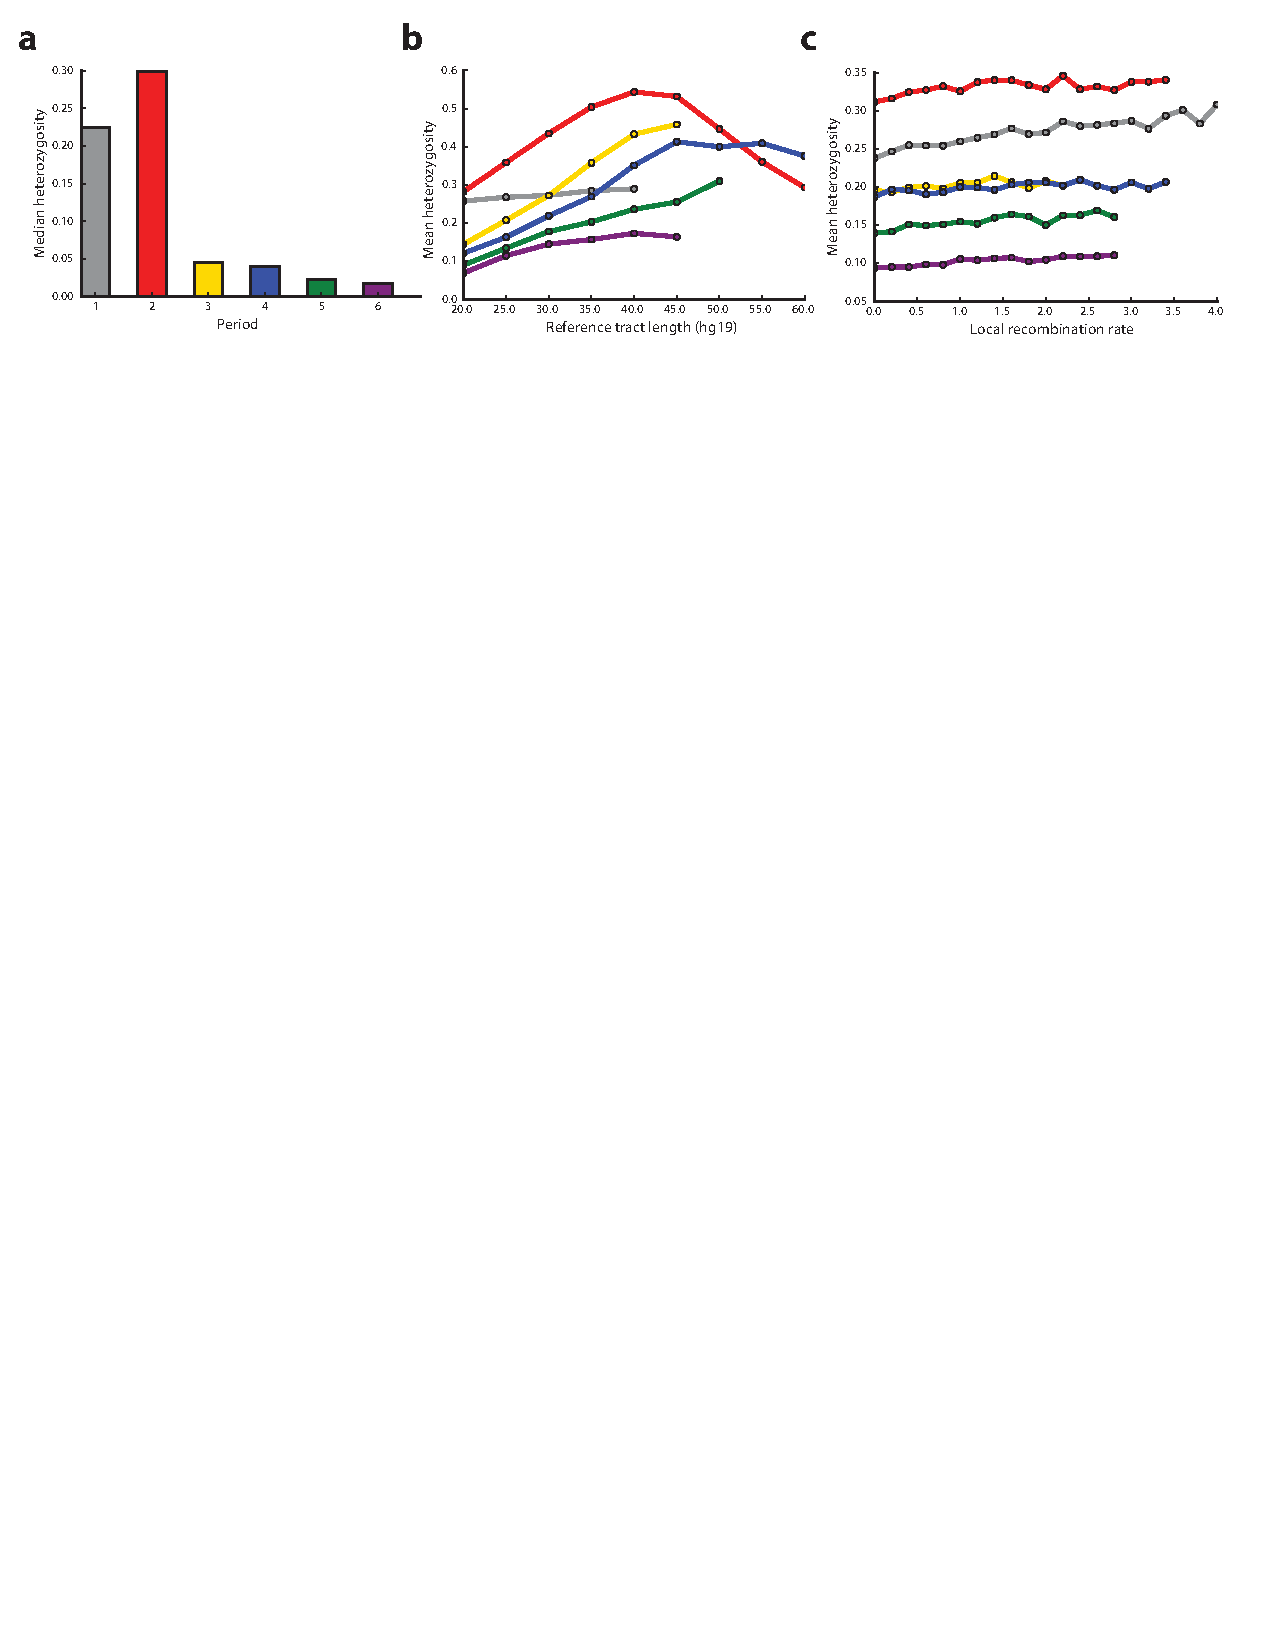
\includegraphics[width=0.8\textwidth]{Figures/App3/Fig4.pdf}
\caption{\textbf{Sequence determinants of STR variation.} \textbf{a}. Median heterozygosity by motif length. STRs with longer motif lengths tend to be less polymorphic. \textbf{b., c}. Mean heterozygosity as a function of reference track length and local recombination rate (gray = homopolymers, red = dinucleotides, yellow = trinucleotides, blue = tetranucleotides, green = pentanucleotides, purple = hexanucleotides).}
\end{figure}

\section{Potential loss-of-function variants at STRs}
We used our catalog to identify STRs in coding regions with common loss-of-function (LoF) variants, which we identified as frameshifting variants in coding exons as defined by Refseq. We restricted to alleles found in at least 10 individuals. Seventeen loci with potential common frameshifts passed these criteria, five of which have a frameshift as the major allele (\textbf{Table \ref{tab:sgdptab2}}). Four of the five common LoF alleles with periods 2-6 reported by \cite{WillemsGymrekHighnamEtAl2014}. using an independent dataset are included in our list (\emph{TMEM254, GP6, FAM166B}, and \emph{DCHS2}), and more than half were reported in dbSNP, suggesting that these putative LoF do not represent genotyping errors. 

In 13 of the 17 cases, the potential LoF variant occurs in the last exon of the gene or toward the end of a single-exon gene, reducing its potential impact on protein function. The variants in \emph{TMEM254} and \emph{LFNG} occur in an internal exon. In both cases there are alternative transcript annotations that do not contain the affected exons. The putative LoF variants for \emph{PTEN} and \emph{RYK} occur in the first exons of these genes. On visual inspection, the CCG repeat for \emph{RYK} occurs in a difficult-to-align GC-rich area and likely represents an alignment artifact. The variant in \emph{PTEN} is fixed at a 1bp deletion from the reference sequence adjacent to the CGG repeat. This deletion is annotated as a 1bp intron in Refseq ((\textbf{Figure \ref{fig:sgdpfig5}})). Notably this region is not annotated as coding by Ensembl, Gencode, or UCSC and the frameshift allele is fixed across all samples, suggesting an error in gene annotation. In conclusion, most common STR frameshift variants are unlikely to affect protein function.

\begin{figure}[h!]
\centering
\label{fig:sgdpfig5}
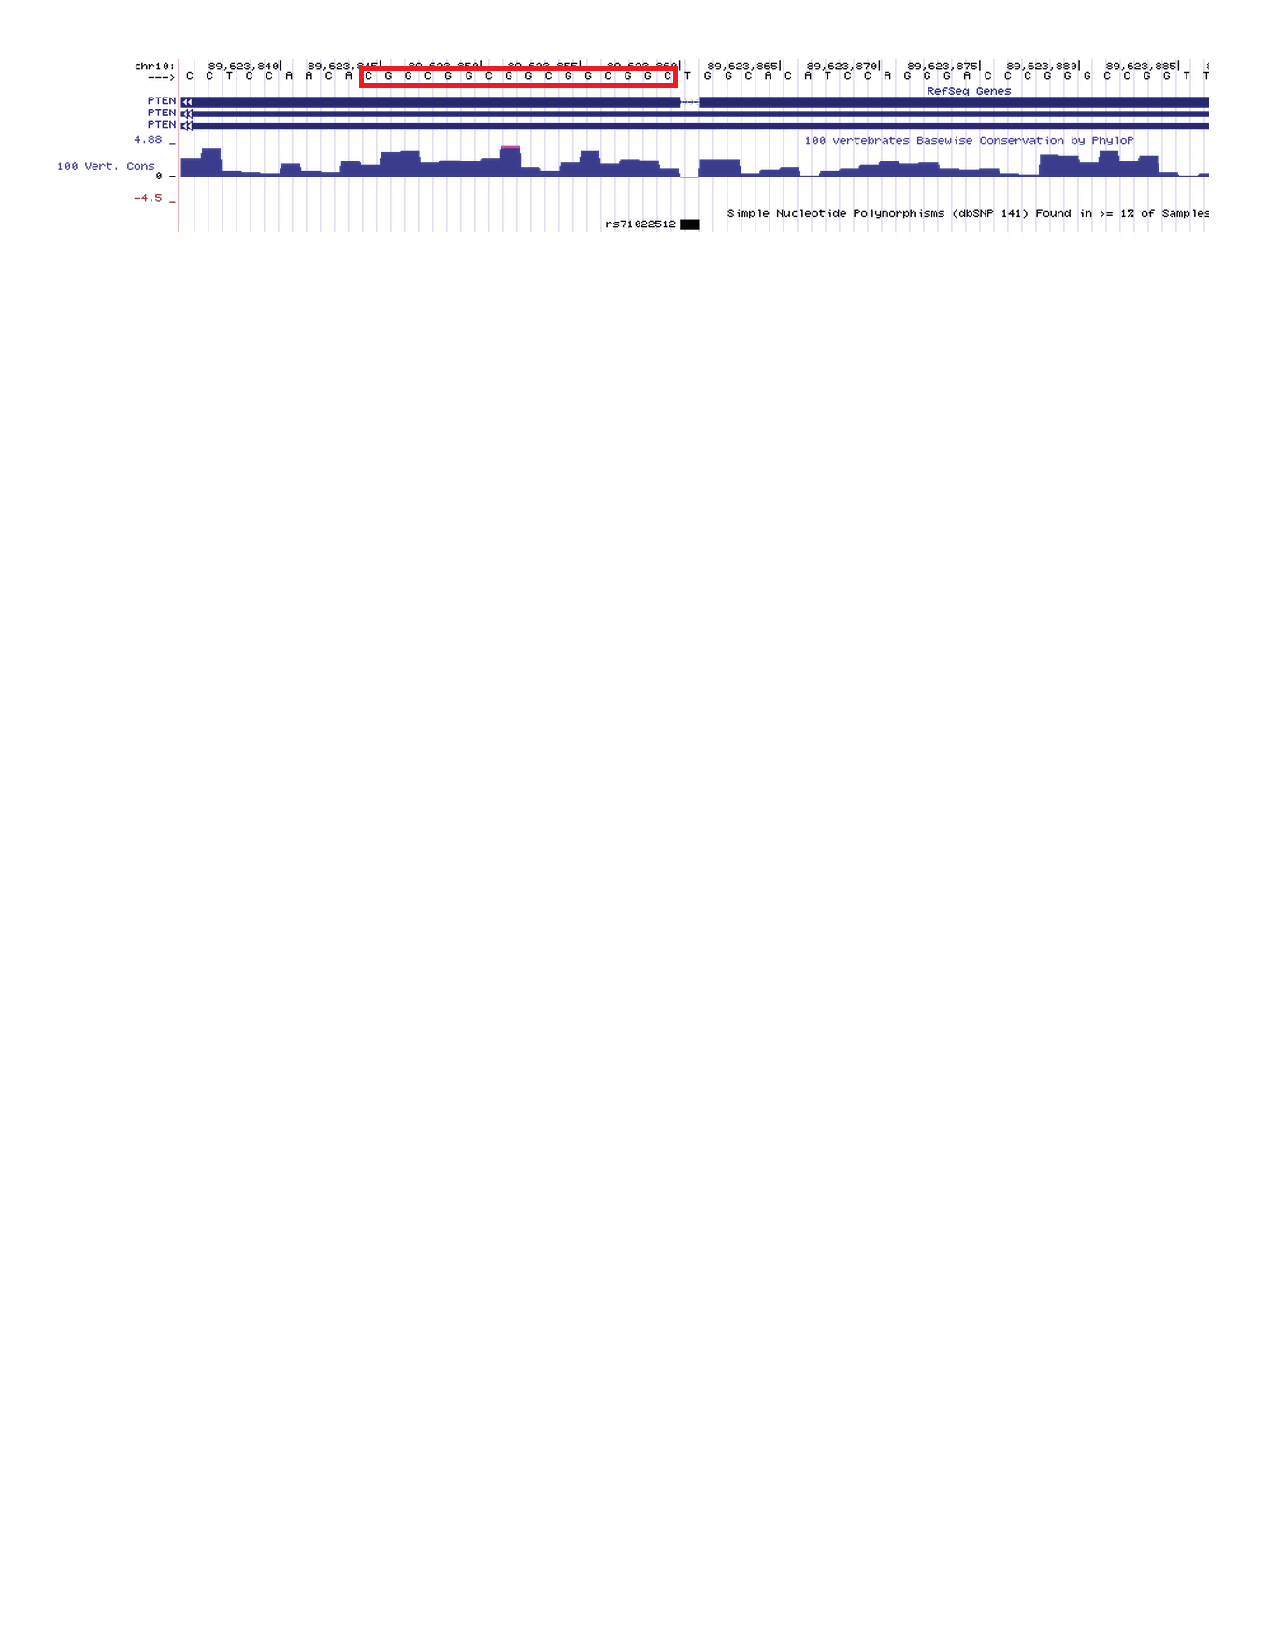
\includegraphics[width=0.9\textwidth]{Figures/App3/Fig5.pdf}
\caption{\textbf{The major allele at an STR in \emph{PTEN} is an apparent frameshift from the reference sequence.} The red box denotes the CGG repeat. The 1bp deletion at the adjacent ``T'' nucleotide is fixed across samples, has poor conservation compared to surrounding bases, and is not annotated as a coding region in other gene annotations, suggesting it may in fact be a misannotation and not a true frameshift variant.}
\end{figure}

\begin{table}[h!]
\centering
\label{tab:sgdptab2}
\begin{adjustbox}{width=1\textwidth}
\begin{tabular}{l l l l l}
\hline
STR Locus & Gene & Motif & LoF & dbSNP \\
\hline
chr13:51530580  & RNASEH2B & A      & 1bp (0.030)                   & rs200320729 (-/A)                      \\
chr14:23528485  & ACIN1$^+$   & AGAGGG & -2bp (0.030)                  &                                        \\
chr10:81841429  & TMEM254$^*$ & AAAG   & -4bp (0.034)                  & rs143538725 (-/AAAG)                   \\
chr3:133969414  & RYK$^+$     & CCG    & 1bp (0.036)                   &                                        \\
chr15:83677271  & C15orf40 & A      & 1bp (0.078)                   &                                        \\
chr19:55526092  & GP6$^*$     & ACAG   & 4bp (0.093)                   & rs138680589 (-/CAGA)                   \\
chr5:147861098  & HTR4$^+$    & AAAAAG & 1bp, -1bp (0.095)             &                                        \\
chr12:55820959  & OR6C76   & A      & -1bp (0.218)                  &                                        \\
chr20:3026346   & GNRH2    & CCCCG  & 5bp (0.320)                   &                                        \\
chr16:58577316  & CNOT1    & A      & -1bp (0.367)                  &                                        \\
chr9:35561913   & FAM166B$^*$ & ACCC   & 1bp, -8bp (0.402)             & rs143266743 (-/CCCACCCT)               \\
chr7:2552851    & LFNG     & ATCC   & 4bp, -4bp (0.422)             &                                        \\
chr6:31380147   & MICA     & AGC    & -1bp, -4bp, 2bp, 11bp (0.810) & rs547446871 (-/G)                      \\
                &          &        &                               & rs41293539 (-/CT/CTGCTGCT/CTGCTGCTGCT) \\
chr4:155244402  & DCHS2$^*$   & AAAC   & -4bp (0.846)                  & rs140019361 (-/TTTG)                   \\
chr10:125780753 & CHST15   & C      & -1bp (0.895)                  & rs5788645 (-/C)                        \\
chr10:89623845  & PTEN     & CCG    & -1bp (1.000)                  & rs71022512 (-/A)                       \\
chr5:72743281   & FOXD1    & CCG    & 2bp (1.000)                   & rs587745355 (-/GC)                    \\
\hline
\end{tabular}
\end{adjustbox}
\caption{\textbf{Common loss-of-function alleles at STRs.} We give the combined allele frequencies of all frameshift alleles for each locus. dbSNP data is from versions 141 and 142. $^*$ entries are LoF alleles previously reported by Willems, et al. $^+$ entries are low confidence alleles likely due to alignment artifacts or stutter errors.}
\end{table}

\section{Conclusion}
We have presented the highest quality catalog of STR variation to date, which can serve as a gold standard reference panel of STR polymorphisms across diverse populations. Additionally, our dataset provides unprecedented opportunities to study STR variation that were not possible using previous studies either due to the small number of markers or to the low quality of individual genotypes5. Importantly, it contains the first panel of previously inaccessible homopolymer genotypes and allows in-depth study of these extremely polymorphic loci for the first time. We envision that this dataset will be an invaluable resource for future studies of STR polymorphism.
